\section{Mô tả ca sử dụng}

Phần này trình bày chi tiết các ca sử dụng (use case) của hệ thống Smart Gallery, làm rõ tương tác giữa người dùng và hệ thống để đáp ứng các yêu cầu chức năng đã đặc tả. Mỗi ca sử dụng được mô tả theo cấu trúc thống nhất, bao gồm tác nhân, điều kiện tiên quyết, luồng xử lý chính, luồng xử lý thay thế và điều kiện sau khi thực hiện. Việc phân tích các ca sử dụng giúp đảm bảo tính đầy đủ của các tính năng và cung cấp cái nhìn trực quan về cách thức vận hành của ứng dụng từ góc độ người dùng.


% \subsection{Ca sử dụng đăng nhập}
\vspace{0.5cm}

\noindent 
\begin{tabularx}{\linewidth}{| l | X |} 
\hline 
\textbf{Mô tả} & Khi người dùng muốn sử dụng các chức năng yêu cầu quyền đăng nhập. \\ 
\hline 
\textbf{Luồng cơ bản} & 1. Truy cập trang đăng nhập \\ 
                      & 2. Nhập thông tin tài khoản (email / mật khẩu) \\ 
                      & 3. Điều hướng đến trang home - danh sách ảnh. \\ 
\hline 
\textbf{Luồng thay thế} & Người dùng nhập sai thông tin tài khoản: \\ 
                       & 1. Hiển thị thông báo lỗi trên form đăng nhập \\ 
\hline 
\textbf{Tiền điều kiện} & Người dùng đã đăng xuất. \\ 
\hline 
\textbf{Hậu điều kiện} & Hệ thống lưu token đăng nhập vào local storage. \\ 
\hline 
\textbf{Yêu cầu phi chức năng} & Hệ thống xử lý đăng nhập không quá 2s. \\ 
\hline 
\end{tabularx}

\vspace{0.8cm}

\noindent 
\begin{tabular}{| c | c |}
    \hline
    \textbf{Biểu đồ hoạt động} & \textbf{Quan hệ} \\ 
    \hline
    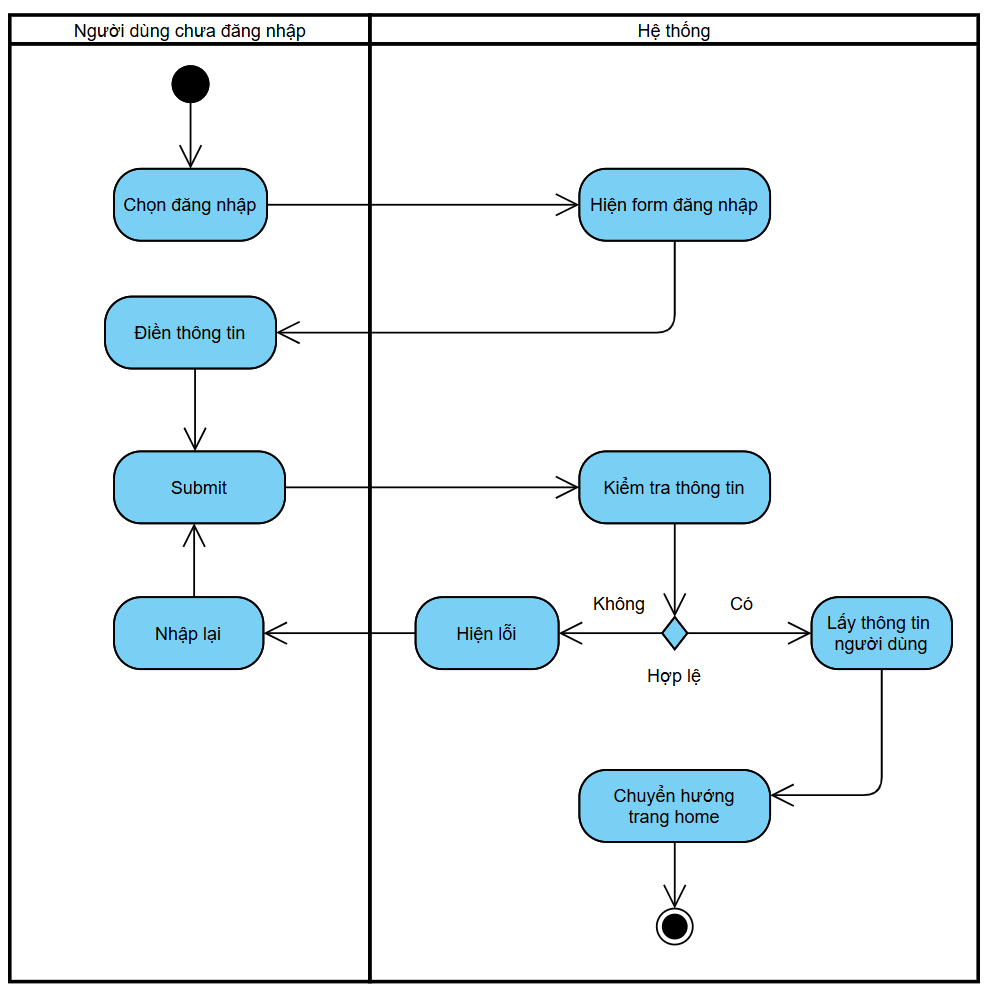
\includegraphics[width=0.45\linewidth]{figures/c3/3-3-1-activity-diagram.png} 
    & 
    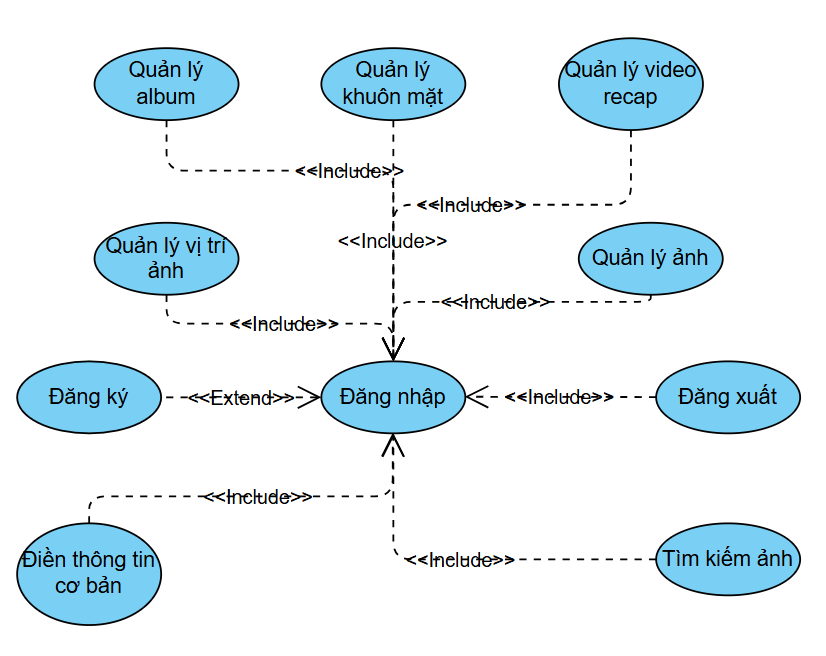
\includegraphics[width=0.45\linewidth]{figures/c3/3-3-1-relationship.png} \\ 
    \hline
\end{tabular}

\begin{figure}[H]
    \centering  
    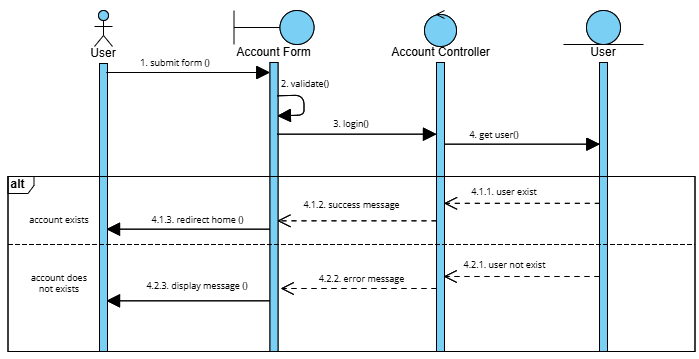
\includegraphics[width=1.1\textwidth]{figures/c3/3-3-1-sequence-diagram.png}
    \caption{Biểu đồ tuần tự ca sử dụng đăng nhập.}
    \label{fig:3-3-1-sequence-diagram}
\end{figure}


% \nopagebreak
% \subsection{Ca sử dụng đăng ký}
\vspace{0.5cm}


\noindent 
\begin{tabularx}{\linewidth}{| l | X |} 
\hline 
\textbf{Mô tả} & Cho phép người dùng tạo một tài khoản trên ứng dụng để sử dụng các chức năng. \\ 
\hline 
\textbf{Luồng cơ bản} & 1. Người dùng truy cập màn hình đăng ký tài khoản. \newline
                       2. Ứng dụng hiển thị giao diện đăng ký tài khoản, yêu cầu người dùng nhập thông tin. \newline
                       3. Người dùng điền tên, email và mật khẩu của tài khoản muốn đăng ký. \newline
                       4. Người dùng nhấn đăng ký để hoàn thành quá trình. \newline
                       5. Hệ thống kiểm tra thông tin người dùng để trả về thông báo phù hợp và điều hướng người dùng đến màn hình điền thông tin cơ bản. \\ 
\hline 
\textbf{Luồng thay thế} &
                       - Nếu có lỗi tại server, hệ thống sẽ không lưu lại thông tin đã nhập vào. \newline
                       - Nếu thông tin nhập vào không hợp lệ sẽ thông báo lỗi để người dùng nhập lại. \\ 
\hline 
\textbf{Tiền điều kiện} & - Màn hình đăng ký đã hiển thị thành công trên ứng dụng. \newline
                       - Tài khoản email đúng định dạng và chưa được đăng ký trước đây. \\ 
\hline 
\textbf{Hậu điều kiện} & - Người đã đăng ký tài khoản có thể sử dụng nó để đăng nhập và thực hiện các chức năng với quyền hạn tương ứng. \newline
                       - Một hồ sơ người dùng được tạo và có thể được chỉnh sửa. \\ 
\hline 
\textbf{Yêu cầu phi chức năng} & Hệ thống xử lý đăng ký không quá 2s \\ 
\hline 
\end{tabularx}

\vspace{0.8cm}

\noindent 
\begin{tabular}{| c | c |}
    \hline
    \textbf{Biểu đồ hoạt động} & \textbf{Quan hệ} \\ 
    \hline
    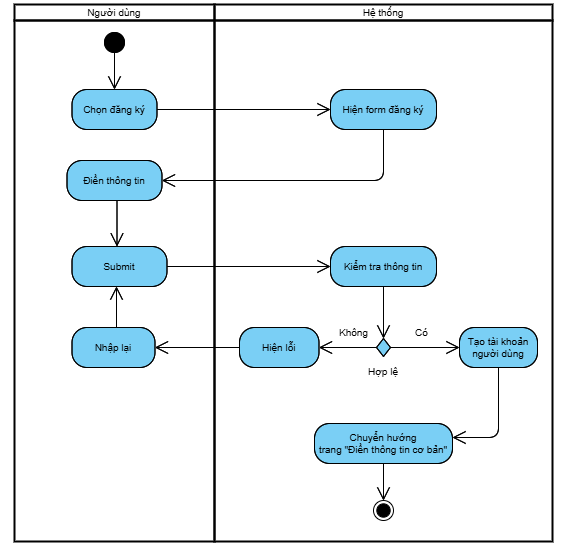
\includegraphics[width=0.45\linewidth]{figures/c3/3-3-2-activity-diagram.png} 
    & 
    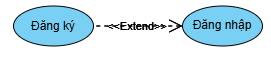
\includegraphics[width=0.4\linewidth]{figures/c3/3-3-2-relationship.png} \\ 
    \hline
\end{tabular}

\begin{figure}[H]
    \centering  
    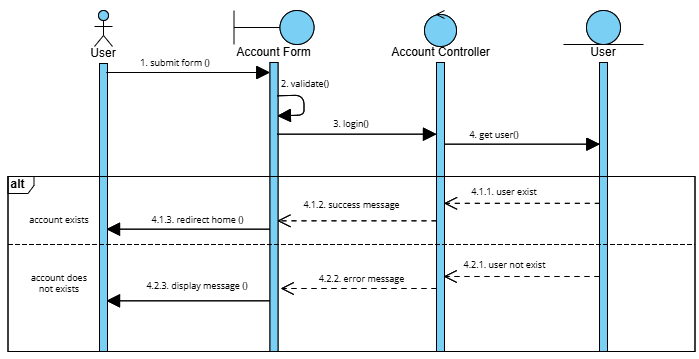
\includegraphics[width=1.1\textwidth]{figures/c3/3-3-1-sequence-diagram.png}
    \caption{Biểu đồ tuần tự ca sử dụng đăng ký.}
    \label{fig:3-3-2-sequence-diagram}
\end{figure}

% \nopagebreak
\subsection{Ca sử dụng điền thông tin cơ bản}

\vspace{0.5cm}


\noindent 
\begin{tabularx}{\linewidth}{| l | X |} 
\hline 
\textbf{Mô tả} & Người dùng cập nhật thông tin cá nhân như ngày sinh, tên, khảo sát, ảnh đại diện và thực hiện 1 số thao tác làm quen với tính năng hệ thống. \\ 
\hline 
\textbf{Luồng cơ bản} & 1. Người dùng đăng ký tài khoản mới. \newline
                       2. Người dùng tải ảnh đại diện lên. \newline
                       3. Người dùng điền tên và ngày sinh. \newline
                       4. Người dùng upload 3 ảnh lên để hệ thống hiển thị và giới thiệu tính năng gán nhãn ảnh. \newline
                       5. Người dùng điền form khảo sát. \newline
                       6. Người dùng bấm nút hoàn thành. \newline
                       7. Hệ thống điều hướng người dùng đến trang chủ của ứng dụng. \\
\hline 
\textbf{Luồng thay thế} &
                       - Nếu thông tin nhập vào không hợp lệ sẽ thông báo lỗi để người dùng nhập lại. \\ 
\hline 
\textbf{Tiền điều kiện} & Người dùng đăng ký tài khoản thành công và chưa hoàn thành điền hết 4 form thông tin cá nhân. \\
\hline 
\textbf{Hậu điều kiện} & - Thông tin cá nhân của người dùng được cập nhật. \newline
                       - Ảnh đại diện và 3 ảnh được upload lên sẽ được hệ thống đưa vào thư viện người dùng. \\ 
\hline 
\textbf{Yêu cầu phi chức năng} & Hệ thống xử lý gán nhãn ảnh không quá 5s \\
\hline 
\end{tabularx}

\vspace{0.8cm}

\noindent 
\begin{tabular}{| c | c |}
    \hline
    \textbf{Biểu đồ hoạt động} & \textbf{Quan hệ} \\ 
    \hline
    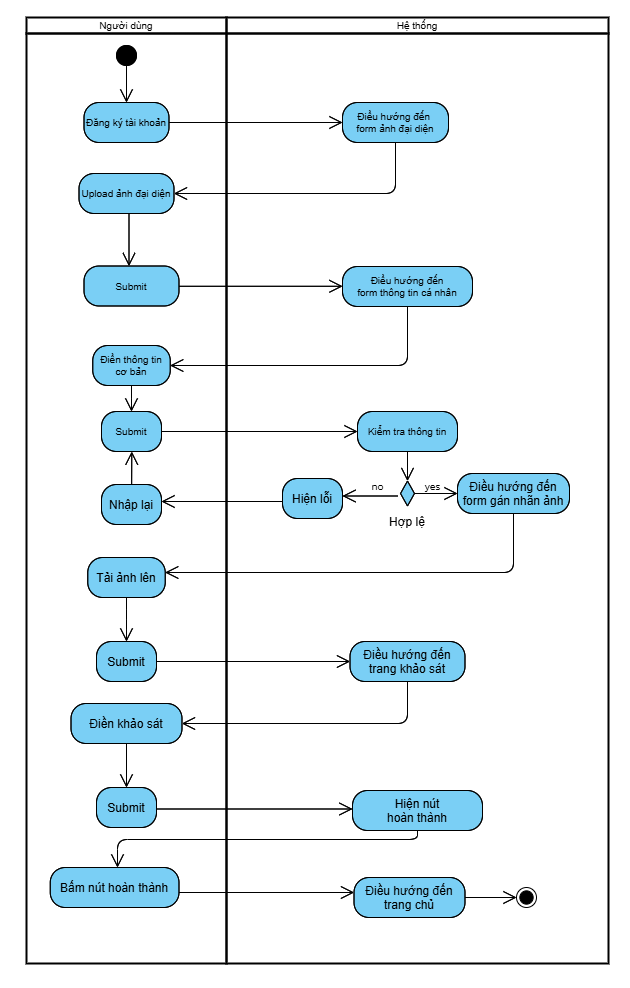
\includegraphics[width=0.6\linewidth]{figures/c3/3-3-3-activity-diagram.png} 
    & 
    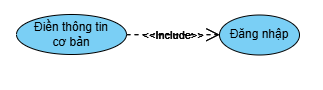
\includegraphics[width=0.35\linewidth]{figures/c3/3-3-3-relationship.png} \\ 
    \hline
\end{tabular}

\begin{figure}[H]
    \centering  
    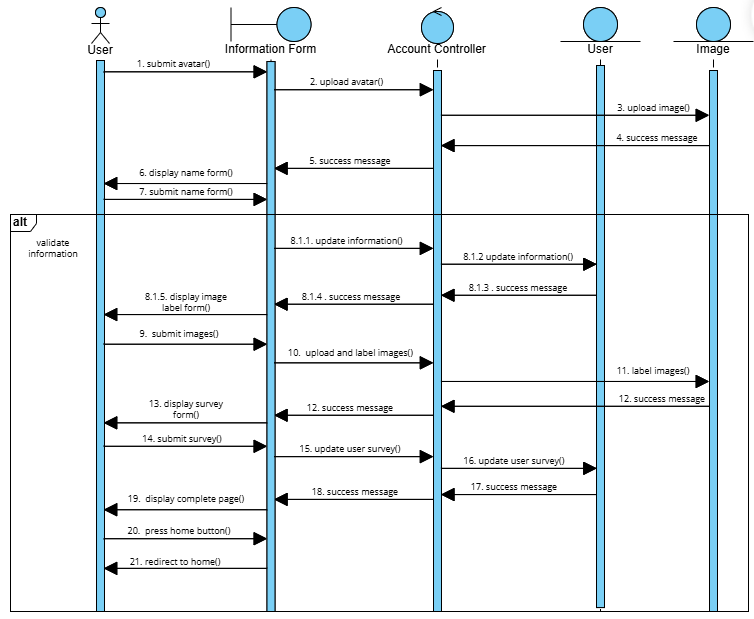
\includegraphics[width=1.1\textwidth]{figures/c3/3-3-3-sequence-diagram.png}
    \caption{Biểu đồ tuần tự ca sử dụng điền thông tin cơ bản.}
    \label{fig:3-3-3-sequence-diagram}
\end{figure}
\nopagebreak
\subsection{Ca sử dụng tải ảnh lên}

\nopagebreak
% \subsection{Ca sử dụng xem chi tiết ảnh}

\vspace{0.5cm}

\noindent 
\begin{tabularx}{\linewidth}{| l | X |} 
\hline 
\textbf{Mô tả} & Người dùng xem thông tin chi tiết của ảnh \\
\hline 
\textbf{Luồng cơ bản} & 1. Người dùng chọn ảnh muốn xem thông tin trong màn hình thư viện. \newline
                       2. Hệ thống hiển thị ảnh ở chế độ toàn màn hình cùng thanh công cụ.\newline
                       3. Người dùng bấm nút xem thêm thông tin ảnh. \newline
                       4. Hệ thống hiển thị các thông tin của ảnh. Bao gồm: tên ảnh, album ảnh thuộc về, kich cỡ, caption ảnh, ngày tải lên, khuôn mặt trong bức ảnh, các nhãn và địa điểm chụp. \\
\hline 
\textbf{Tiền điều kiện} & - Người dùng đăng ký / đăng nhập tài khoản thành công và hoàn thành điền form thông tin cơ bản. \newline
                        - Người dùng đã tải ít nhất 1 ảnh lên thư viện. \\
\hline 
\textbf{Hậu điều kiện} & - Hệ thống hiển thị các thông tin ảnh chi tiết cho người dùng. \\
\hline 
\textbf{Yêu cầu phi chức năng} & Hệ thống truy vấn các thông tin của ảnh không quá 2s. \\
\hline 
\end{tabularx}

\vspace{0.8cm}

\noindent 
\begin{tabular}{| c | c |}
    \hline
    \textbf{Biểu đồ hoạt động} & \textbf{Quan hệ} \\ 
    \hline
    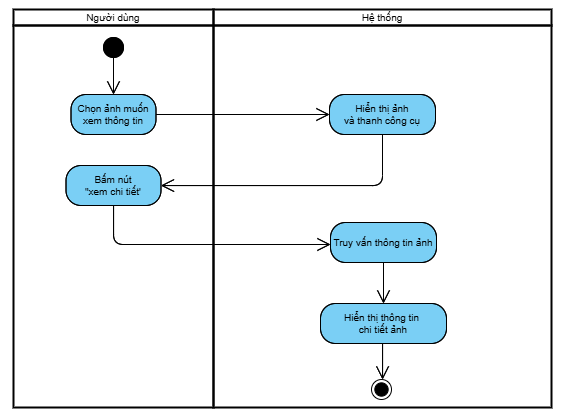
\includegraphics[width=0.6\linewidth]{figures/c3/3-3-5-activity-diagram.png} 
    & 
    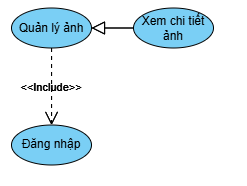
\includegraphics[width=0.35\linewidth]{figures/c3/3-3-5-relationship.png} \\ 
    \hline
\end{tabular}

\begin{figure}[H]
    \centering  
    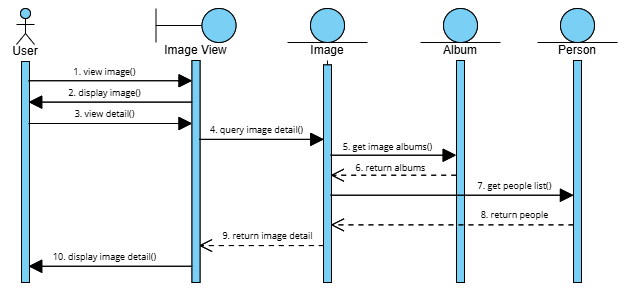
\includegraphics[width=1\textwidth]{figures/c3/3-3-5-sequence-diagram.png}
    \caption{Biểu đồ tuần tự ca sử dụng xem chi tiết ảnh.}
    \label{fig:3-3-5-sequence-diagram}
\end{figure}

% \nopagebreak
% \subsection{Ca sử dụng thao tác trên ảnh}

\vspace{0.5cm}

\noindent 
\begin{tabularx}{\linewidth}{| l | X |} 
\hline 
\textbf{Mô tả} & Người dùng thao tác với ảnh trong thư viện: yêu thích, chỉnh sửa caption, tải ảnh xuống và xóa ảnh. \\
\hline 
\textbf{Luồng cơ bản} & 1. Người dùng chọn ảnh muốn thao tác tron thư viện. \newline
                       2. Hệ thống hiển thị ảnh ở chế độ toàn màn hình cùng thanh công cụ.\newline
                       3. Người dùng bấm nút yêu thích ảnh. \newline
                       4. Hệ thống đánh dấu ảnh là yêu thích và cập nhật giao diện. \newline
                       5. Người dùng bấm nút chỉnh sửa caption ảnh. \newline
                       6. Hệ thống hiển thị form chỉnh sửa caption ảnh. \newline
                       7. Người dùng nhập caption mới và bấm nút lưu. \newline
                       8. Hệ thống cập nhật caption ảnh và cập nhật lại giao diện. \newline
                       9. Người dùng bấm nút tải ảnh xuống. \newline
                       10. Hệ thống lưu ảnh vào máy người dùng và hiển thị thông báo thành công. \newline
                       11. Người dùng bấm nút xóa ảnh. \newline
                       12. Hệ thống xóa ảnh trong thư viện, hiển thị thông báo thành công và hiển thị ảnh tiếp theo. \\
\hline 
\textbf{Luồng thay thế} &
                        - Người dùng không nhập caption / caption ảnh không thay đổi so với caption cũ \\ 
\hline 
\textbf{Hậu điều kiện} & - Hệ thống cập nhật các thông tin của ảnh được update: yêu thích, caption, ... \\
\hline 
\textbf{Yêu cầu phi chức năng} & Hệ thống xử lý mỗi thao tác không quá 1s. \\
\hline 
\end{tabularx}

\vspace{0.8cm}

\noindent 
\begin{tabular}{| c | c |}
    \hline
    \textbf{Biểu đồ hoạt động} & \textbf{Quan hệ} \\ 
    \hline
    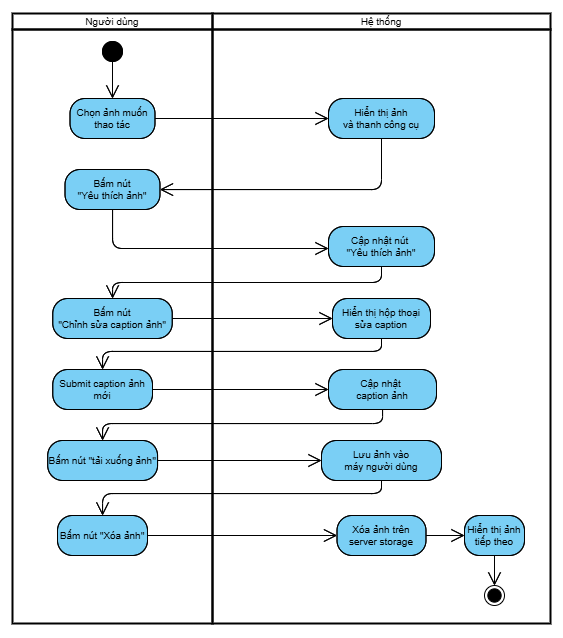
\includegraphics[width=0.6\linewidth]{figures/c3/3-3-6-activity-diagram.png} 
    &  
    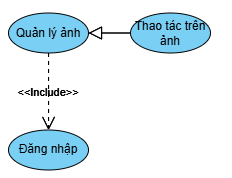
\includegraphics[width=0.35\linewidth]{figures/c3/3-3-6-relationship.png} \\ 
    \hline
\end{tabular}

\begin{figure}[H]
    \centering  
    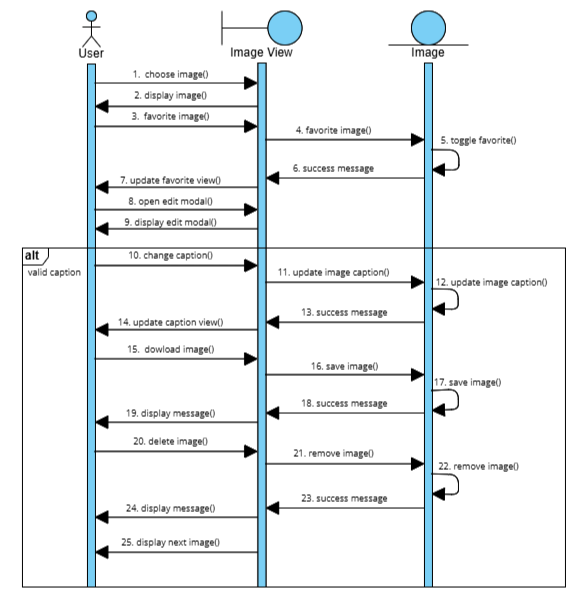
\includegraphics[width=1\textwidth]{figures/c3/3-3-6-sequence-diagram.png}
    \caption{Biểu đồ tuần tự ca sử dụng thao tác trên ảnh.}
    \label{fig:3-3-6-sequence-diagram}
\end{figure}

% \nopagebreak
\subsection{Ca sử dụng tạo album}

Người dùng sau khi tải ảnh lên hệ thống có thể tạo album để phân loại ảnh theo chủ đề. Hệ thống sẽ sắp xếp ảnh theo thứ tự thời gian tải lên và hiển thị dưới dạng lưới cho người dùng.

Mô tả chi tiết cho ca sử dụng tạo album được thể hiện ở Bảng \ref{tab:create-album-usecase} dưới đây. Kèm theo là Bảng \ref{tab:create-album-usecase-activity} về biểu đồ hoạt động, quan hệ và Hình \ref{fig:3-3-7-sequence-diagram} về biểu đồ tuần tự của ca sử dụng này. 

\noindent 

\begin{table}[H]
\centering
\begin{tabularx}{\linewidth}{| l | X |} 
\hline 
\textbf{Mô tả} & Người dùng tạo album mới trong thư viện ảnh. \\
\hline 
\textbf{Luồng cơ bản} & 1. Người dùng bấm nút tạo album trong thanh công cụ ở dưới màn hình. \newline
                       2. Hệ thống hiển thị hộp thoại điền tên album.\newline
                       3. Người dùng nhập tên album và bấm nút tạo album. \newline
                       4. Hệ thống hiển thị hộp thoại chọn ảnh trong album từ danh sách những ảnh người dùng đã tải lên hệ thống.\newline
                       5. Người dùng chọn những ảnh muốn đưa vào album và bấm nút tạo album. \newline
                       6. Hệ thống tạo album và hiển thị giao diện danh sách ảnh trong album và tiêu đề. \\
\hline 
\textbf{Tiền điều kiện} & - Người dùng đã đăng nhập vào hệ thống. \newline
                           - Người dùng đã có ảnh trong thư viện. \\
\hline
\textbf{Hậu điều kiện} & - Hệ thống cập nhật album mới vào danh sách các album đang có để hiển thị trong trang danh sách album. \\
\hline 
\textbf{Yêu cầu phi chức năng} & Hệ thống xử lý tạo album không quá 2s. \\
\hline 
\end{tabularx}
\caption{Mô tả chi tiết ca sử dụng tạo album.}
\label{tab:create-album-usecase}
\end{table}

\vspace{0.8cm}

\noindent 
\begin{table}[H]
\centering
\begin{tabular}{| c | c |}
    \hline
    \textbf{Biểu đồ hoạt động} & \textbf{Quan hệ} \\ 
    \hline
    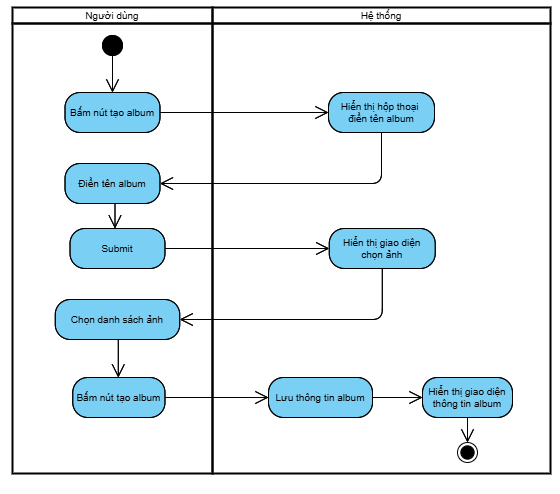
\includegraphics[width=0.6\linewidth]{figures/c3/3-3-7-activity-diagram.png} 
    &  
    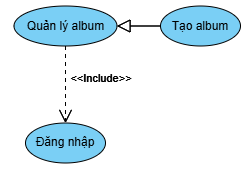
\includegraphics[width=0.35\linewidth]{figures/c3/3-3-7-relationship.png} \\ 
    \hline
\end{tabular}
\caption{Biểu đồ hoạt động và quan hệ ca sử dụng tạo album.}
\label{tab:create-album-usecase-activity}
\end{table}

\noindent
\begin{figure}[H]
    \centering  
    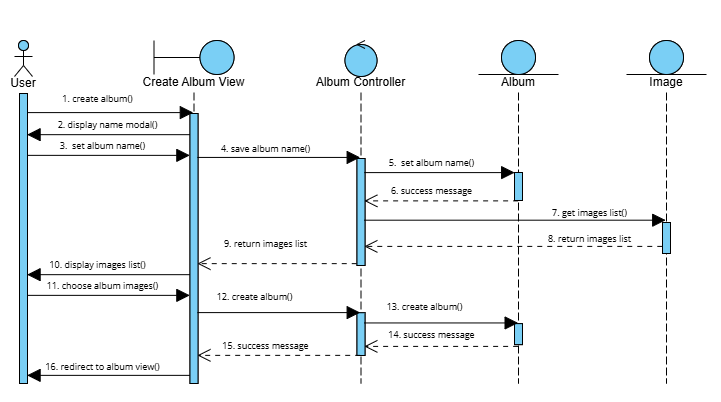
\includegraphics[width=1\textwidth]{figures/c3/3-3-7-sequence-diagram.png}
    \caption{Biểu đồ tuần tự ca sử dụng tạo album.}
    \label{fig:3-3-7-sequence-diagram}
\end{figure}

\nopagebreak
\subsection{Ca sử dụng xem danh sách video recap}

Người dùng sau khi gửi yêu cầu tạo video có thể theo dõi trạng thái video của mình trong danh sách video. Hệ thống sẽ cập nhật trạng thái và tiến độ của video theo thời gian thực.  

Mô tả chi tiết cho ca sử dụng xem danh sách video recap được thể hiện ở Bảng \ref{tab:view-video-recap-usecase} dưới đây. Kèm theo là Bảng \ref{tab:view-video-recap-usecase-activity} về biểu đồ hoạt động, quan hệ và Hình \ref{fig:3-3-8-sequence-diagram} về biểu đồ tuần tự của ca sử dụng này. 

\noindent 

\begin{table}[H]
\centering
\caption{Mô tả chi tiết ca sử dụng xem danh sách video recap}
\label{tab:view-video-recap-usecase}
\begin{tabularx}{\linewidth}{| l | X |} 
\hline 
\textbf{Mô tả} & Người dùng xem danh sách và trạng thái của các video đã tạo. \\
\hline 
\textbf{Luồng cơ bản} & 1. Người dùng bấm nút xem danh sách video ở thanh công cụ dưới màn hình. \newline
                       2. Hệ thống điều hướng đến trang danh sách video và hiển thị.\newline
                       3. Người dùng nhập tên album và bấm nút tạo album. \\
\hline 
\textbf{Tiền điều kiện} & - Người dùng đã đăng nhập vào hệ thống. \newline
                            - Người dùng đã tạo ít nhất 1 video recap. \\
\textbf{Hậu điều kiện} & - Người dùng có thể xem chi tiết trạng thái render của từng video. \newline
                        - Người dùng có thể xem những video đã render xong. \newline
                        - Hệ thống cập nhật trạng thái và tiến độ của các video trong thời gian thực. \\
\hline 
\textbf{Yêu cầu phi chức năng} & - Hệ thống lấy danh sách video không quá 2s. \newline
                        - Hệ thống cập nhật trạng thái video thời gian thực, không quá 0.5s. \\   
\hline 
\end{tabularx}
\end{table}

\vspace{0.8cm}

\noindent 
\begin{table}[H]
\centering
\caption{Biểu đồ hoạt động và quan hệ ca sử dụng xem danh sách video recap}
\label{tab:view-video-recap-usecase-activity}
\begin{tabular}{| c | c |}
    \hline
    \textbf{Biểu đồ hoạt động} & \textbf{Quan hệ} \\ 
    \hline
    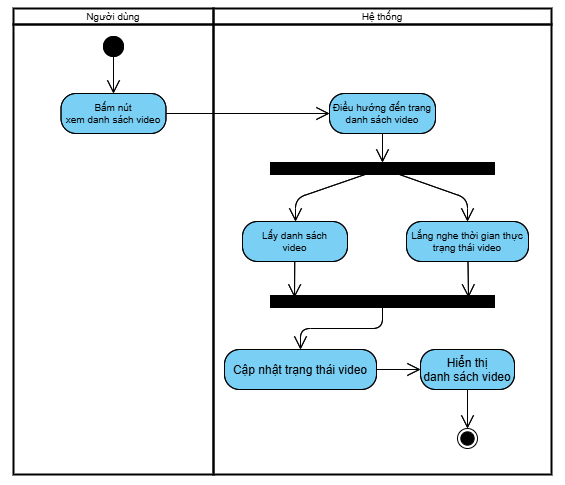
\includegraphics[width=0.6\linewidth]{figures/c3/3-3-8-activity-diagram.png} 
    &  
    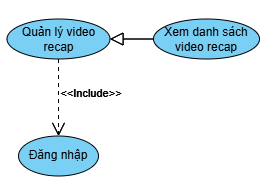
\includegraphics[width=0.35\linewidth]{figures/c3/3-3-8-relationship.png} \\ 
    \hline
\end{tabular}
\end{table}

\begin{figure}[ht]
    \centering  
    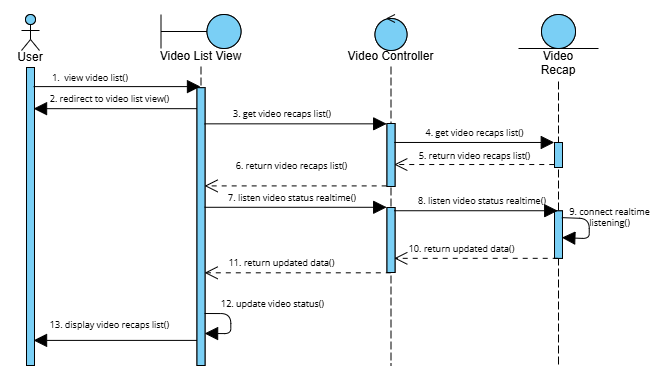
\includegraphics[width=1\textwidth]{figures/c3/3-3-8-sequence-diagram.png}
    \caption{Biểu đồ tuần tự ca sử xem danh sách video recap.}
    \label{fig:3-3-8-sequence-diagram}
\end{figure}
\nopagebreak
\subsection{Ca sử dụng tạo video recap}

\vspace{0.2cm}

\noindent 
\begin{tabularx}{\linewidth}{| l | X |} 
\hline 
\textbf{Mô tả} & Người dùng tạo video recap từ các ảnh trong thư viện. \\
\hline 
\textbf{Luồng cơ bản} & 1. Người dùng bấm nút tạo video recap từ thanh công cụ ở dưới màn hình. \newline
                       2. Hệ thống hiển thị giao diện chọn danh sách ảnh.\newline
                       3. Người dùng chọn ảnh trong danh sách ảnh đã tải lên hệ thống. \newline
                       4. Người dùng chọn ảnh trong danh sách ảnh của máy người dùng.\newline
                       5. Người dùng bấm submit danh sách ảnh. \newline
                       6. Hệ thống tạo kịch bản cho video và những tùy chỉnh mặc định cho video từ danh sách ảnh: style khung ảnh, nhạc nền, chất lượng video, thời lượng video, chủ đề video. \newline
                       7. Người dùng chỉnh các tùy chỉnh cho video: style khung ảnh, nhạc nền, chất lượng video, thời lượng video, chủ đề video. \newline
                       8. Người dùng bấm submit để tạo video. \newline
                       9. Hệ thống tạo video từ danh sách ảnh và kịch bản đã chọn. \newline
                       10. Hệ thống điều hướng đến màn hình xem trạng thái tạo video theo thời gian thực. \\
\hline 
\textbf{Tiền điều kiện} & - Người dùng đã đăng nhập vào hệ thống. \newline
                            - Người dùng đã có ảnh trong thư viện. \\
\hline
\textbf{Hậu điều kiện} & - Hệ thống hiển thị trạng thái và tiến độ tạo video theo thời gian thực. \newline
                         - Người dùng quay về màn hình danh sách video để theo dõi trạng thái video đã tạo. \\
\hline 
\textbf{Yêu cầu phi chức năng} & - Hệ thống xử lý tạo kịch bản video không quá 20s. \newline 
                                 - Hệ thống tạo video không quá 5 phút. \newline
                                 - Hệ thống cập nhật trạng thái video theo thời gian thực. \\
\hline 
\end{tabularx}

\vspace{0.8cm}

\noindent 
\begin{tabular}{| c | c |}
    \hline
    \textbf{Biểu đồ hoạt động} & \textbf{Quan hệ} \\ 
    \hline
    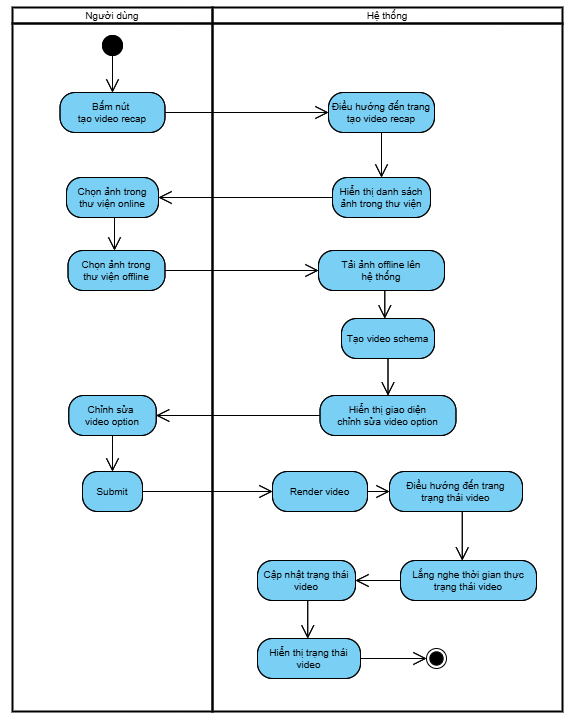
\includegraphics[width=0.6\linewidth]{figures/c3/3-3-9-activity-diagram.png} 
    &  
    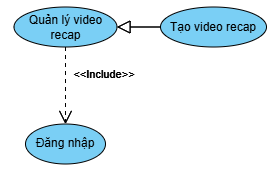
\includegraphics[width=0.35\linewidth]{figures/c3/3-3-9-relationship.png} \\ 
    \hline
\end{tabular}

\begin{figure}[H]
    \centering  
    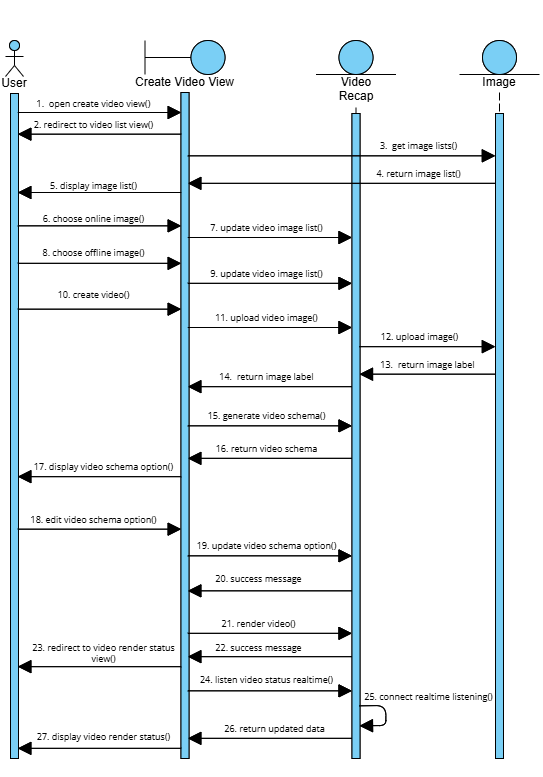
\includegraphics[width=1.1\textwidth]{figures/c3/3-3-9-sequence-diagram.png}
    \caption{Biểu đồ tuần tự ca sử dụng tạo video recap.}
    \label{fig:3-3-9-sequence-diagram}
\end{figure}

\nopagebreak
\subsection{Ca sử dụng xem danh sách khuôn mặt}

\vspace{0.5cm}

\noindent 
\begin{tabularx}{\linewidth}{| l | X |} 
\hline 
\textbf{Mô tả} & Người dùng muốn xem các danh sách khuôn mặt xuất hiện trong các bức ảnh tải lên. \\
\hline 
\textbf{Luồng cơ bản} & 1. Người dùng bấm vào ô khám phá khuôn mặt. \newline
                       2. Hệ thống lấy dữ liệu những khuôn mặt trong ảnh người dùng. \newline
                       3. Hệ thống lấy dữ liệu nhóm khuôn mặt đã được tạo trước đó. \newline
                       4. Hệ thống thực hiện phân loại và so sánh nhóm khuôn mặt mới với nhóm khuôn mặt cũ. \newline
                       5. Hệ thống hiển thị danh sách các khuôn mặt và tên gọi (nếu có). \\
\hline
\textbf{Luồng thay thế} & 2a. Nếu có những nhóm khuôn mặt có sẵn thì hệ thống so sánh nhóm mới với nhóm cũ. Và sau đó nhóm mới sẽ thay thế nhóm cũ nếu phù hợp. \\
\hline
\textbf{Tiền điều kiện} & - Người dùng đã đăng nhập vào hệ thống. \newline
                           - Hệ thống đã phân loại khuôn mặt trong ảnh. \\
\textbf{Hậu điều kiện} & - Hệ thống hiển thị trạng thái và tiến độ tạo video theo thời gian thực. \newline
                         - Người dùng quay về màn hình danh sách video để theo dõi trạng thái video đã tạo. \\
\hline 
\textbf{Yêu cầu phi chức năng} & -Hệ thống xử lý nhóm khuôn mặt không quá 20s. \\
\hline 
\end{tabularx}

\vspace{0.8cm}

\noindent 
\begin{tabular}{| c | c |}
    \hline
    \textbf{Biểu đồ hoạt động} & \textbf{Quan hệ} \\ 
    \hline
    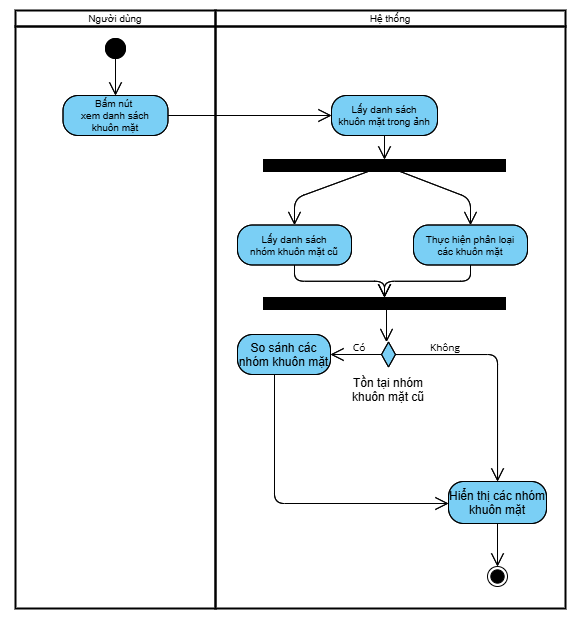
\includegraphics[width=0.6\linewidth]{figures/c3/3-3-10-activity-diagram.png} 
    &  
    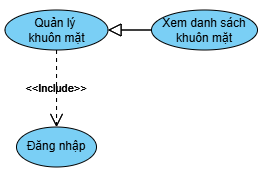
\includegraphics[width=0.35\linewidth]{figures/c3/3-3-10-relationship.png} \\ 
    \hline
\end{tabular}

\begin{figure}[H]
    \centering  
    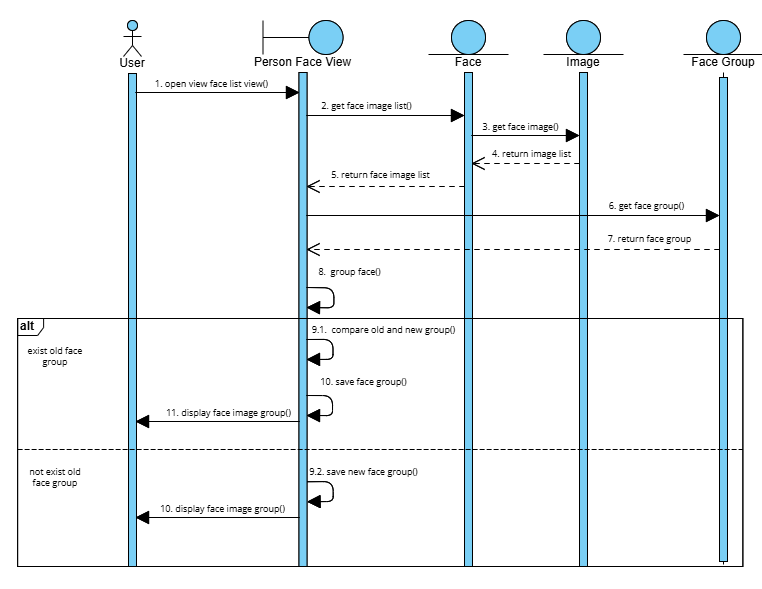
\includegraphics[width=1.1\textwidth]{figures/c3/3-3-10-sequence-diagram.png}
    \caption{Biểu đồ tuần tự ca sử dụng xem danh sách khuôn mặt.}
    \label{fig:3-3-10-sequence-diagram}
\end{figure}
\nopagebreak
% \subsection{Ca sử dụng xem ảnh theo khuôn mặt}


% \nopagebreak
% \subsection{Ca sử dụng đổi tên khuôn mặt}

\vspace{0.5cm}

\noindent 
\begin{tabularx}{\linewidth}{| l | X |} 
\hline 
\textbf{Mô tả} & Người dùng đổi tên của nhóm khuôn mặt đã được hệ thống phân loại. \\
\hline 
\textbf{Luồng cơ bản} & 1. Người dùng bấm vào nút đổi tên khuôn mặt. \newline
                       2. Hệ thống hiển thị hộp thoại đổi tên. \newline
                       3. Người dùng nhập tên khuôn mặt mới và submit. \newline
                       5. Hệ thống cập nhật tên và giao diện. \\
\hline
\textbf{Luồng thay thế} & - Tên mới không được trùng với tên nhóm cũ / trống. \\
\textbf{Tiền điều kiện} & - Người dùng đã đăng nhập vào hệ thống. \newline
                          - Hệ thống đã hoàn thành phân loại khuôn mặt trên ảnh. \\
\textbf{Hậu điều kiện} & - Người dùng có thể chọn ảnh để xem chi tiết. \newline
                          - Người dùng có thể đổi tên khuôn mặt. \\
\hline 
\textbf{Yêu cầu phi chức năng} & -Hệ thống cập nhật tên khuôn mặt không quá 1s. \\
\hline 
\end{tabularx}

\vspace{0.8cm}

\noindent 
\begin{tabular}{| c | c |}
    \hline
    \textbf{Biểu đồ hoạt động} & \textbf{Quan hệ} \\ 
    \hline
    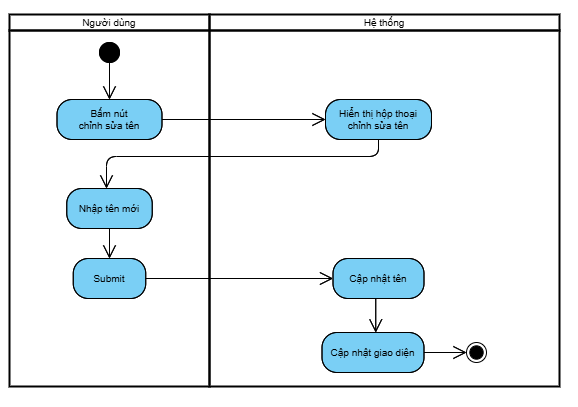
\includegraphics[width=0.6\linewidth]{figures/c3/3-3-12-activity-diagram.png} 
    &  
    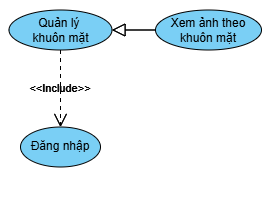
\includegraphics[width=0.35\linewidth]{figures/c3/3-3-12-relationship.png} \\ 
    \hline
\end{tabular}

\begin{figure}[H]
    \centering  
    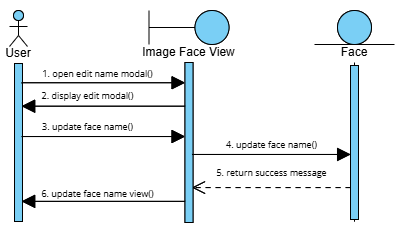
\includegraphics[width=1\textwidth]{figures/c3/3-3-12-sequence-diagram.png}
    \caption{Biểu đồ tuần tự ca sử dụng đổi tên khuôn mặt.}
    \label{fig:3-3-12-sequence-diagram}
\end{figure}
% \nopagebreak
% \subsection{Ca sử dụng xem địa điểm chụp ảnh}
% \nopagebreak
\subsection{Ca sử dụng xem ảnh theo địa điểm}
\nopagebreak
\subsection{Ca sử dụng thêm vị trí cho ảnh}

Người dùng có thể thêm thủ công vị trí cho ảnh đã tải lên trong thư viện của mình. Hệ thống sẽ tự động lấy vị trí hiện tại của người dùng (nếu được cấp quyền) và hiển thị trên bản đồ. Người dùng có thể chọn vị trí trên bản đồ hoặc tìm kiếm địa điểm để thêm vị trí cho ảnh.

Mô tả chi tiết cho ca sử dụng thêm vị trí cho ảnh được thể hiện ở Bảng \ref{tab:add-location-usecase} dưới đây. Kèm theo là Bảng \ref{tab:add-location-usecase-activity} về biểu đồ hoạt động, quan hệ và Hình \ref{fig:3-3-15-sequence-diagram} về biểu đồ tuần tự của ca sử dụng này. 

\noindent 
\begin{table}[H]
\centering
\begin{tabular}{| c | c |}
    \hline
    \textbf{Biểu đồ hoạt động} & \textbf{Quan hệ} \\ 
    \hline
    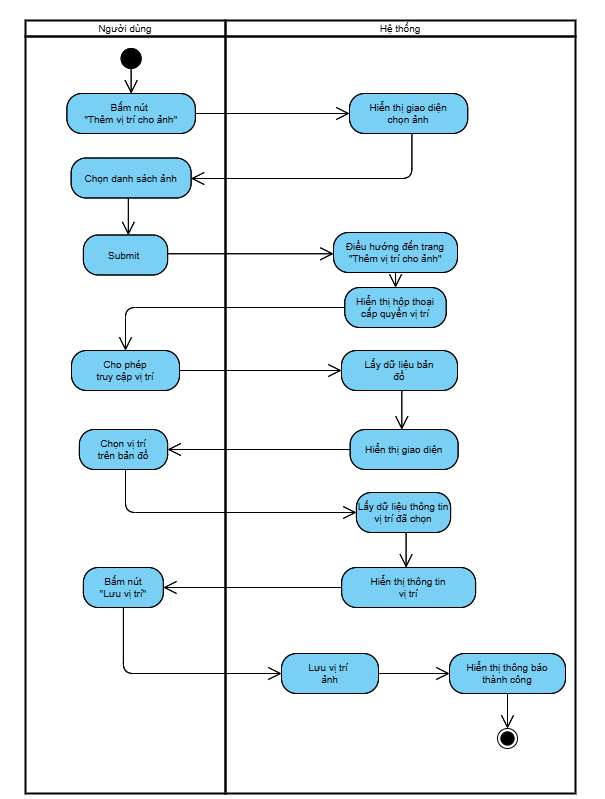
\includegraphics[width=0.6\linewidth]{figures/c3/3-3-15-activity-diagram.png} 
    &  
    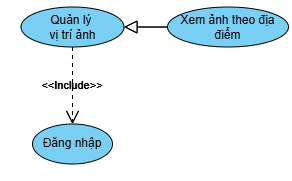
\includegraphics[width=0.35\linewidth]{figures/c3/3-3-15-relationship.png} \\ 
    \hline
\end{tabular}
\caption{Biểu đồ hoạt động và quan hệ ca sử dụng thêm vị trí cho ảnh.}
\label{tab:add-location-usecase-activity}
\end{table}

\noindent 
\begin{table}[H]
\centering
\begin{tabularx}{\linewidth}{| l | X |} 
\hline 
\textbf{Mô tả} & Người dùng thêm vị trí cho ảnh. \\
\hline 
\textbf{Luồng cơ bản} & 1. Người dùng chọn nút thêm vị trí cho ảnh ở thanh công cụ dưới màn hình. \newline
                       2. Hệ thống điều hướng đến trang thêm vị trí cho ảnh. \newline
                       3. Hệ thống hiển thị hộp thoại cấp quyền thông tin vị trí hiện tại. \newline
                       4. Người dùng cấp quyền truy cập vị trí hiện tại. \newline
                       5. Hệ thống lấy thông tin vị trí hiện tại của người dùng và hiển thị trên bản đồ. \newline
                       6. Người dùng chọn vị trí trên bản đồ. \newline
                       7. Người dùng bấm nút xác nhận để thêm vị trí cho ảnh. \newline
                       8. Hệ thống lưu vị trí cho ảnh và hiển thị thông báo thành công. \\
\hline
\textbf{Luồng thay thế} & - Người dùng tìm kiếm địa điểm thay vì tự chọn vị trí thủ công trên bản đồ. \newline
                          - Hệ thống không lấy được dữ liệu địa điểm từ vị trí người dùng chọn trên bản đồ. \\
\hline
\textbf{Tiền điều kiện} & - Người dùng đã đăng nhập vào hệ thống. \newline
                          - Có ít nhất 1 bức ảnh đã tải lên trong thư viện. \\
\hline
\textbf{Hậu điều kiện} & - Người dùng có thể xem vị trí hiện tại của bản thân. \newline
                          - Người dùng có thể xem thông tin chi tiết của vị trí vừa chọn. \\
\hline 
\textbf{Yêu cầu phi chức năng} & - Hệ thống lấy dữ liệu của địa điểm không quá 2s. \newline
                           - Hệ thống lấy được dữ liệu hiện tại vị trí người dùng (nếu được cấp quyền). \\
\hline 
\end{tabularx}
\caption{Mô tả chi tiết ca sử dụng thêm vị trí cho ảnh.}
\label{tab:add-location-usecase}
\end{table}


\begin{figure}[H]
    \centering  
    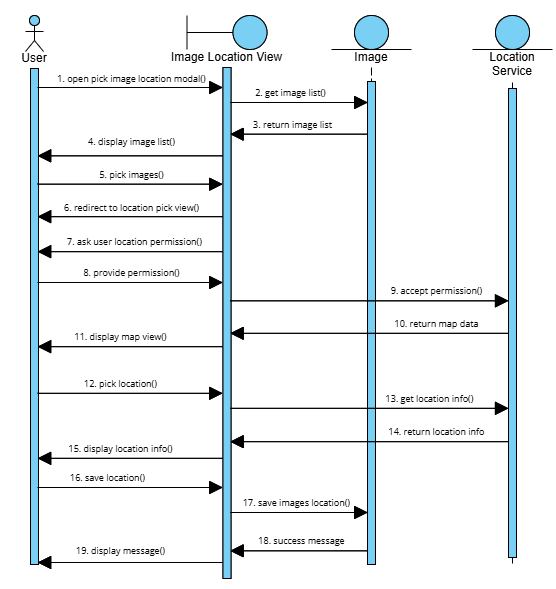
\includegraphics[width=1.1\textwidth]{figures/c3/3-3-15-sequence-diagram.png}
    \caption{Biểu đồ tuần tự ca sử dụng thêm vị trí cho ảnh.}
    \label{fig:3-3-15-sequence-diagram}
\end{figure}
\nopagebreak
\subsection{Ca sử dụng tìm kiếm hình ảnh}

\vspace{0.5cm}

\noindent 
\begin{tabularx}{\linewidth}{| l | X |} 
\hline 
\textbf{Mô tả} & Người dùng tìm kiếm ảnh với những option hệ thống cung cấp. \\
\hline 
\textbf{Luồng cơ bản} & 1. Người dùng bấm vào nút tìm kiếm ở thanh công cụ dưới màn hình. \newline
                       2. Hệ thống điều hướng đến trang tìm kiếm. \newline
                       3. Hệ thống hiển thị các gợi ý về bộ lọc tìm kiếm (thời gian, albums, tên khuôn mặt, tên ảnh, địa điểm, truy vấn AI) và lịch sử tìm kiếm. \newline
                       4. Người dùng gõ từ khóa muốn tìm kiếm. \newline
                       5. Hệ thống hiển thị các gợi ý về bộ lọc có liên quan đến từ khóa tìm kiếm (thời gian, albums, tên khuôn mặt, tên ảnh, địa điểm, truy vấn AI). \newline
                       6. Người dùng chọn gợi ý tìm kiếm khớp với từ khóa muốn tìm. \newline
                       7. Hệ thống lưu lịch sử tìm kiếm và hiển thị kết quả theo dạng danh sách. \\
\hline
\textbf{Luồng thay thế} & - Người dùng tìm kiếm bằng giọng nói thay vì gõ từ khóa. \newline
                           - Người dùng không gõ từ khóa mà chọn gợi ý tìm kiếm. \\
\hline
\textbf{Tiền điều kiện} & - Người dùng đã đăng nhập vào hệ thống. \newline
                          - Có ít nhất 1 bức ảnh đã tải lên trong thư viện. \\
\hline
\textbf{Hậu điều kiện} & - Người dùng có thể xem thêm thông tin chi tiết về ảnh đã tìm kiếm. \newline
                          - Người dùng có thể xóa bộ lọc tìm kiếm. \\
\hline 
\textbf{Yêu cầu phi chức năng} & - Hệ thống lấy truy vấn ảnh không quá 2s. \newline
                            - Hệ thống hiển thị gợi ý tìm kiếm không quá 1s. \\
\hline 
\end{tabularx}

\vspace{0.8cm}

\noindent 
\begin{tabular}{| c | c |}
    \hline
    \textbf{Biểu đồ hoạt động} & \textbf{Quan hệ} \\ 
    \hline
    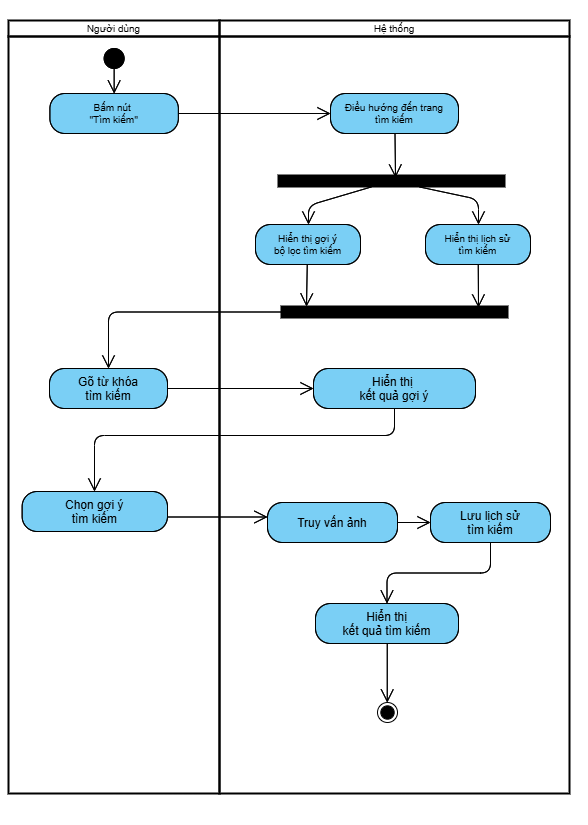
\includegraphics[width=0.6\linewidth]{figures/c3/3-3-16-activity-diagram.png} 
    &  
    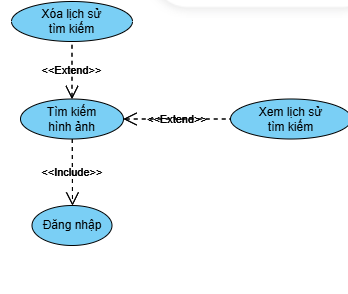
\includegraphics[width=0.35\linewidth]{figures/c3/3-3-16-relationship.png} \\ 
    \hline
\end{tabular}

\begin{figure}[H]
    \centering  
    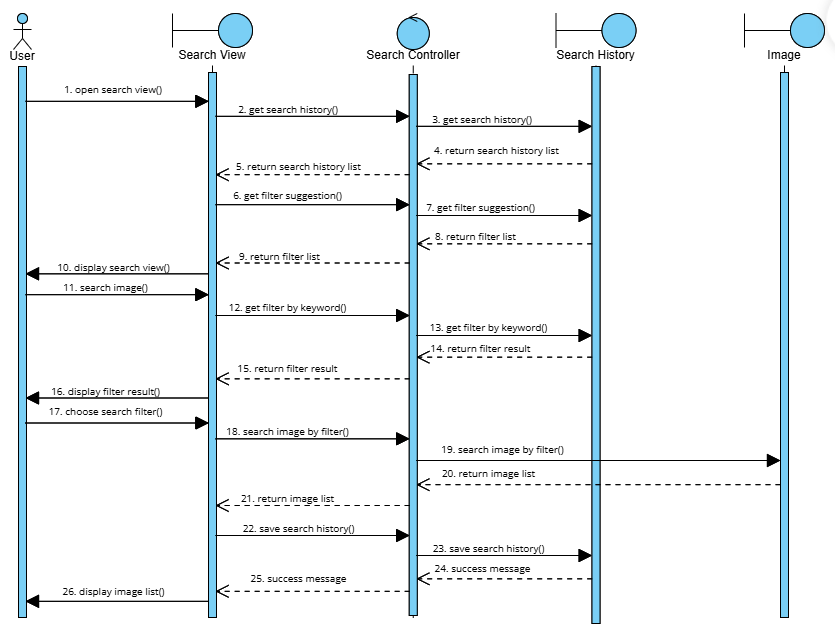
\includegraphics[width=1.1\textwidth]{figures/c3/3-3-16-sequence-diagram.png}
    \caption{Biểu đồ tuần tự ca sử dụng tìm kiếm hình ảnh.}
    \label{fig:3-3-16-sequence-diagram}
\end{figure}
\nopagebreak
% 
\subsection{Ca sử dụng tìm kiếm hình ảnh}

% \nopagebreak